

%\setcounter{chapter}{-1}


\chapter{Множества}

\lesson{1}{08.09.2023}{Операции над множествами}

\section{Операции над множествами}


Офыволфывводфыв


ЛОлвоылфовлы


\begin{theorem}
    Теорема о чем-то
\end{theorem}

\begin{proof}
    Доказательство
\end{proof}

\begin{definition}
    Определение
\end{definition}

\begin{note}

\end{note}


\begin{notation}
    
\end{notation}

\begin{eg}
Пример
\end{eg}

\begin{enumerate}
    \item Что-то
    \item Что-то 2
    \item ФВЫ
    фвывфы

    фывфвы

    \item вфывыф
\end{enumerate}

\begin{itemize}
    \item Что-то
    \item Что-то 2
    \item ФВЫ
    фвывфы

    фывфвы

    \item вфывыф
\end{itemize}


вфыровфыв $f(x) = 10$ выофовфырвфы

% Множеств

$\R \N \Q$

% Греческие символы

$\alpha \beta \chi \psi$

% Операции с множесмтвами

$\cup \cap \subset \in \setminus $

% Палочка сверху

$\overline{asdas}$

$\triangle$

% Степени и то что снизу

$ A_{B_{b_h}}^{123} $

% Математические операции

\begin{theorem}
    

$\frac{123}{456}$

$\log_{123} dasdsa$


$\sum_{n = 1}^{dsads}$

$\int_{123132}^{132312}$

$f(10) \to 321312123$

% кванторы

$\exists \exists! \forall$

% Что-то рядом с чертой

$|_{123}^{123}$

$\wedge \vee \lor \land \leftrightarrow \Leftrightarrow \longleftrightarrow \Updownarrow \Downarrow $


\end{theorem}


\begin{figure}[H]
    \centering
    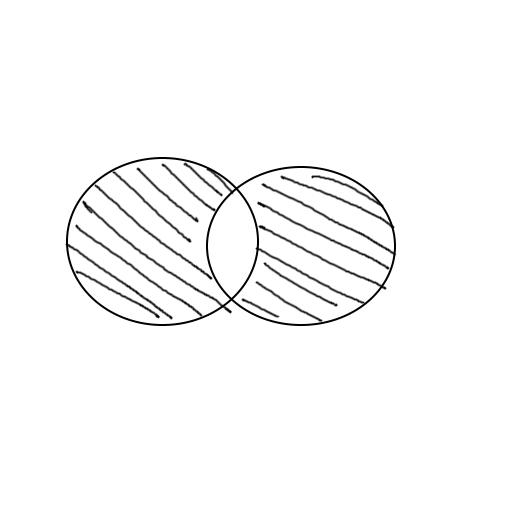
\includegraphics[width=\linewidth]{1.png}
    
    
    \label{fig:1}
\end{figure}